\subsection{Laue-Aufnahme}
\subsubsection{Bestimmung der Millerindizes}
Es war uns leider nicht möglich, die Aufnahme einzuscannen. Deswegen haben wir sie mit einem Lineal photographiert. Das Bild ist in Abb. \ref{fig:laue_raw} zu sehen. Der Abstand beträgt $L = 10\si{\milli\meter}$\\

\begin{figure}
\centering
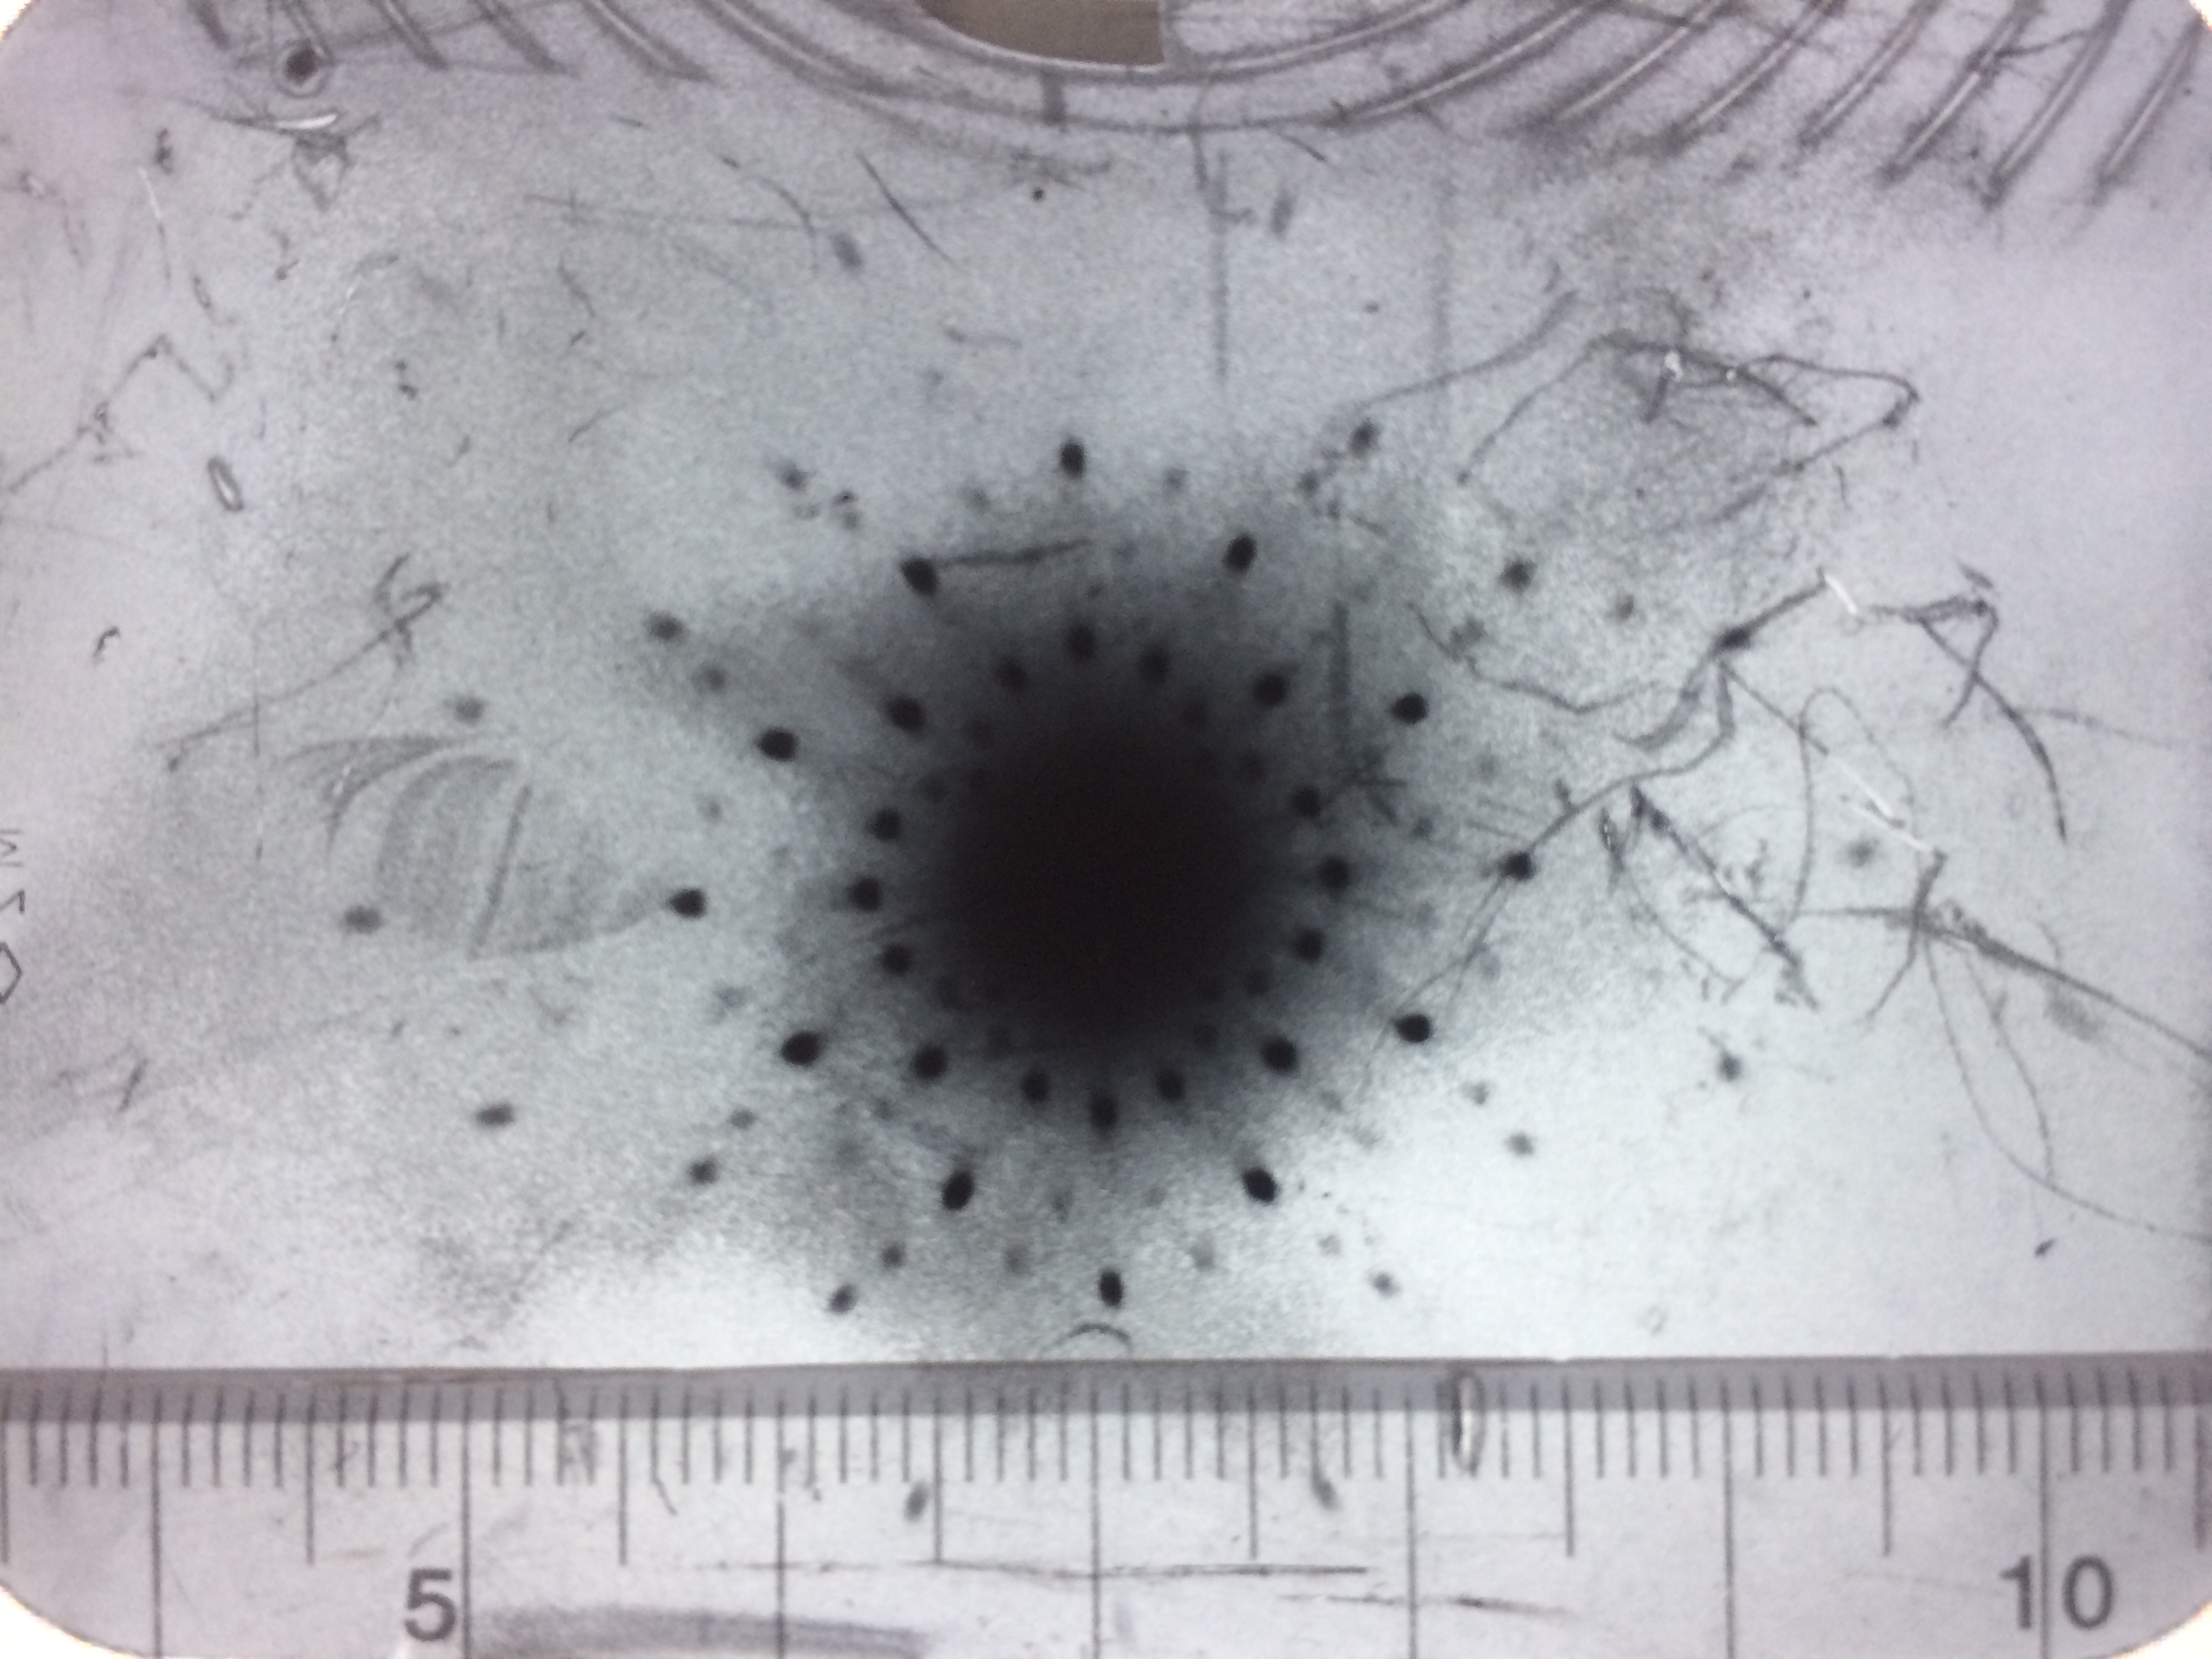
\includegraphics[scale=0.1]{data/laue/laue.jpeg}
\caption{Bild der Laue-Aufnahme}
\label{fig:laue_raw}
\end{figure}

\begin{figure}
\centering
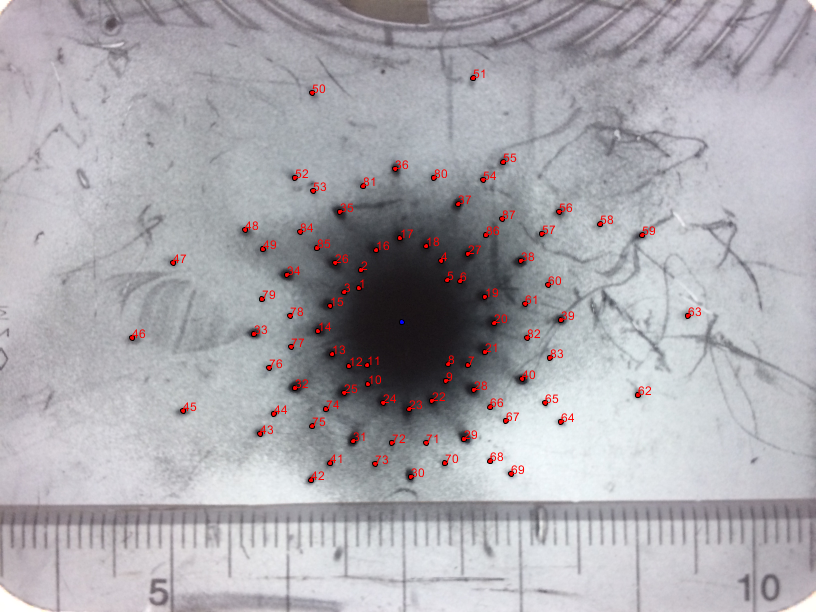
\includegraphics[scale=0.6]{data/laue/draw/laue_before.png}
\caption{Bestimmte Reflexe (blau: Mitte, rot: Reflexe)}
\label{fig:laue_points}
\end{figure}

Mithilfe des Lineals konnten wir die Pixel in die eigentlichen Abstände umrechnen (1px = $0,0214765\si{\milli\meter}$). In dem Bild haben wir nun die Position der erkennbaren Reflexe bestimmt (siehe Abb. \ref{fig:laue_points} und Tab. \ref{tab:coords}). Der Fehler hierbei beträgt $\Delta x, \Delta y = 0,5 \si{\milli\meter}$. Der Mittelpunkt wurde zu $x_0 = (34,534 \pm 2)\si{\milli\meter}, y_0 = (27,662 \pm 2)\si{\milli\meter}$ bestimmt. Die Koordinaten $x\ind{Q}$ und $y\ind{Q}$ der Reflexe ergeben sich nun durch:
\begin{align*}
x\ind{Q} &= x - x_0\\
y\ind{Q} &= y - y_0
\end{align*}
Der Fehler ist $\Delta x\ind{Q}, \Delta y\ind{Q} = \si{2,06 \milli\meter}$.\\
Die Bestimmung der Millerindizes erfolgt anders als im Praktikumsheft beschrieben. Unsere Auswertung basiert auf Gl. \ref{eq:alpha}. Daraus kann man sich aus einer gegebenen Menge $(h,k,l)$ $\alpha$ berechnen und damit auch $x\ind{Q},y\ind{Q},z\ind{Q}$.\\ 

Um nun die Millerindizes den Reflexen zuzuordnen, iterieren wir über die Millerindizes\footnote{Dazu beginnen wir mit $l=1$ und inkrementieren $l$ immer um 1 bis zu einer oberen Grenze $a \in \mathbb{N}$. Die Indizes $h$ und $k$ laufen dann jeweils im Bereich $-a \leq h,k \leq a$ und sind entweder gerade oder ungerade, je nachdem welche Parität $l$ besitzt. Da nach \ref{eq:zq} $z\ind{Q} > 0$ ist und $l > 0$, muss $\alpha > 0$ sein}. Zu jedem Trippel an Indizes berechnen wir $\alpha$. Ist $\alpha < 0$ so verwerfen wir das Trippel. Ansonsten kann man sich aus $\alpha$ die zu erwartende Position des Reflexes berechnen ($x\ind{Q}\upd{theo} = \alpha h$, $y\ind{Q}\upd{theo} = \alpha k$). Wir weisen dem Reflex, der sich am nächsten am berechnetem Punkt befindet, die entsprechenden Millerindizes zu. Ist der Punkt mehrmals am nächsten an einem berechneten Punkt, so werden im die Indizes zugewiesen, bei denen der Abstand am geringsten ist.\\

Das wichtigste bei dieser Methode ist, dass man die obere Schranke $a$ für $h,k,l$ richtig wählt. Wählt man sie zu klein, so werden nur wenige Reflexe zugewiesen. Wählt man sie hingegen zu groß, dann gibt es in der Umgebung eines Reflexes viele mögliche Trippel die in Betracht kommen. Aufgrund des unvermeidlichen Fehlers von $x\ind{Q}, y\ind{Q}$, ist die Chance groß einem Reflex die falschen Indizes zuzuweisen.\\

\begin{figure}
\centering
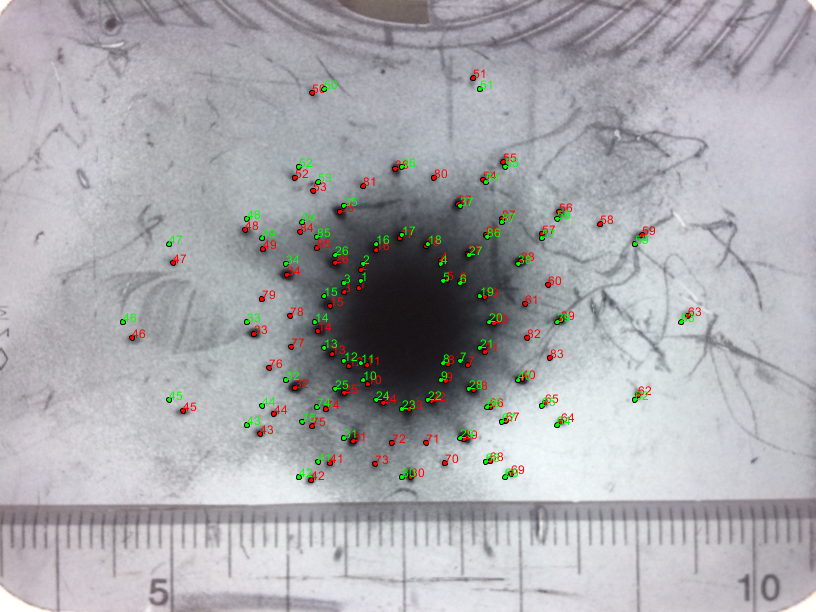
\includegraphics[scale=0.6]{data/laue/draw/laue.png}
\caption{Gemessene (rot) und zugeordnete Reflexe (grün)}
\label{fig:laue_calc}
\end{figure}

Wir haben uns dazu entschieden, $a = 6$ zu wählen. Damit werden fast alle Reflexe zugewiesen, aber die Reflexe liegen auch noch nicht so dicht, dass falsche Indizes zugewiesen werden. Die Millerindizes ist in Tab. \ref{tab:coords} angegeben. In Abb. \ref{fig:laue_calc} sind die berechneten Reflexe dargestellt. Diese liegen in der Nähe der zugewiesenen Reflexe, man kann aber erkennen, dass das Bild leicht verschoben, verzerrt und verdreht ist. Da wir aber davon ausgehen, dass die Reflexe trotzdem richtig zugeordnet worden, haben wir darauf verzichtet, dass Bild zu entzerren und die Berechnungen zu wiederholen. Mit den Formeln \ref{eq:theta} - \ref{eq:d} haben wir noch den Glanzwinkel $\theta$, den Netzebenenabstand $d$ und die Wellenlänge $\lambda$ bestimmt (Gitterkonstante NaCl: $a_0 = 564,00 \si{\pico\meter}$ \cite{wiki_nacl}). Bei den Werten haben wir keine Fehler berechnet, da wir einen möglichen Fehler auf den Millerschen Indizes nicht abschätzen können. Die Wellenlängen liegen im Bereich $40 - 130$, also im Bereich für Röntgenstrahlen.

\subsubsection{Diskussion der Fehler der Millerindizes}
Um zu bestimmen, inwiefern Indizes falsch bestimmt werden hätten können, wurden in Abb. \ref{fig:laue_theo6} alle möglichen Reflexe mit $|h|,|k|,|l| \leq a = 6$ zusammen mit den gemessenen Reflexen dargestellt. Man kann gut erkennen, dass es in der Umgebung aller gemessener Punkte nur einen theoretischen Punkt gibt, der in Frage kommen könnte. Trotzdem wurden fast alle Reflexe bestimmt. Würde man $a = 12$ setzen, so ergäbe sich Abb. \ref{fig:laue_theo12}. Jetzt kann man die Reflexe nicht mehr identifizieren. Es ist also prinzipiell möglich, dass der Reflex auch von einer anderen Netzebene stammen könnte. Allerdings müsste man dann auch noch weitere Reflexe auf dem Bild erkennen können. Da man diese nicht erkennen kann, gehen wir davon aus, dass man im Grunde nur Reflexe mit $|h|,|k|,|l| \leq a = 6$ erkennen kann und somit die Millerindizes korrekt bestimmt wurden.

\begin{figure}
\centering
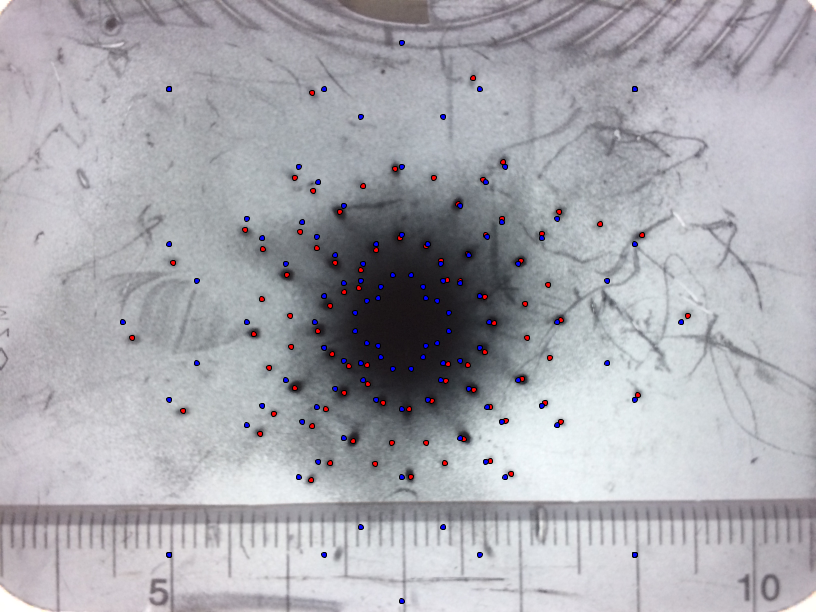
\includegraphics[scale=0.6]{data/laue/draw/laue_theo6.png}
\caption{Gemessene (rot) und berechnete Reflexe (blau) für $a = 6$}
\label{fig:laue_theo6}
\end{figure}

\begin{figure}
\centering
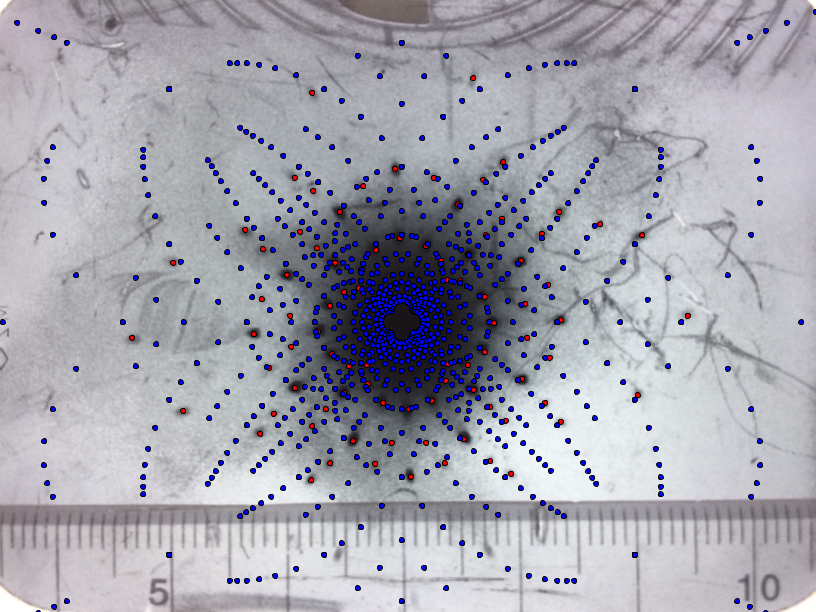
\includegraphics[scale=0.6]{data/laue/draw/laue_theo12.png}
\caption{Gemessene (rot) und berechnete Reflexe (blau)für $a = 12$}
\label{fig:laue_theo12}
\end{figure}

\begin{table}
\centering
\caption{Bestimmte Koordinaten der Reflexe (relativ zur linken oberen Ecke)}
\label{tab:coords}
\begin{tabular}{ccccccccc}
\toprule
Reflex & $x/\si{\milli\meter}$ & $y/\si{\milli\meter}$ & $h$ & $k$ & $l$ & $\theta$ & $d/\si{\pico\meter}$ & $\lambda/\si{\pico\meter}$\\
\midrule
1 & 30,84 & 24,741 & -3 & -3 & 1 & 0,23 & 129,40 & 59,37\\
2 & 31,012 & 23,195 & -4 & -6 & 2 & 0,27 & 75,37 & 40,29\\
3 & 29,552 & 25,085 & -6 & -4 & 2 & 0,27 & 75,37 & 40,29\\
4 & 37,885 & 22,421 & 4 & -6 & 2 & 0,27 & 75,37 & 40,29\\
5 & 38,4 & 24,054 & 3 & -3 & 1 & 0,23 & 129,40 & 59,37\\
6 & 39,517 & 24,14 & 6 & -4 & 2 & 0,27 & 75,37 & 40,29\\
7 & 40,204 & 31,356 & 6 & 4 & 2 & 0,27 & 75,37 & 40,29\\
8 & 38,486 & 31,27 & 3 & 3 & 1 & 0,23 & 129,40 & 59,37\\
9 & 38,314 & 32,73 & 4 & 6 & 2 & 0,27 & 75,37 & 40,29\\
10 & 31,613 & 32,988 & -4 & 6 & 2 & 0,27 & 75,37 & 40,29\\
11 & 31,528 & 31,356 & -3 & 3 & 1 & 0,23 & 129,40 & 59,37\\
12 & 29,981 & 31,442 & -6 & 4 & 2 & 0,27 & 75,37 & 40,29\\
13 & 28,521 & 30,411 & -3 & 1 & 1 & 0,31 & 170,06 & 102,55\\
14 & 27,318 & 28,435 & -6 & 0 & 2 & 0,32 & 89,18 & 56,40\\
15 & 28,349 & 26,287 & -3 & -1 & 1 & 0,31 & 170,06 & 102,55\\
16 & 32,301 & 21,477 & -1 & -3 & 1 & 0,31 & 170,06 & 102,55\\
17 & 34,362 & 20,446 & 0 & -6 & 2 & 0,32 & 89,18 & 56,40\\
18 & 36,596 & 21,133 & 1 & -3 & 1 & 0,31 & 170,06 & 102,55\\
19 & 41,664 & 25,514 & 3 & -1 & 1 & 0,31 & 170,06 & 102,55\\
20 & 42,438 & 27,748 & 6 & 0 & 2 & 0,32 & 89,18 & 56,40\\
21 & 41,664 & 30,239 & 3 & 1 & 1 & 0,31 & 170,06 & 102,55\\
22 & 37,111 & 34,448 & 1 & 3 & 1 & 0,31 & 170,06 & 102,55\\
23 & 35,136 & 35,136 & 0 & 6 & 2 & 0,32 & 89,18 & 56,40\\
24 & 32,902 & 34,62 & -1 & 3 & 1 & 0,31 & 170,06 & 102,55\\
25 & 29,552 & 33,761 & -4 & 4 & 2 & 0,34 & 94,00 & 62,67\\
26 & 28,779 & 22,593 & -4 & -4 & 2 & 0,34 & 94,00 & 62,67\\
27 & 40,204 & 21,82 & 4 & -4 & 2 & 0,34 & 94,00 & 62,67\\
28 & 40,719 & 33,503 & 4 & 4 & 2 & 0,34 & 94,00 & 62,67\\
29 & 39,86 & 37,713 & 2 & 4 & 2 & 0,42 & 115,13 & 94,00\\
30 & 35,307 & 40,977 & 0 & 4 & 2 & 0,46 & 126,12 & 112,80\\
31 & 30,325 & 37,885 & -2 & 4 & 2 & 0,42 & 115,13 & 94,00\\
32 & 25,342 & 33,332 & -4 & 2 & 2 & 0,42 & 115,13 & 94,00\\
33 & 21,82 & 28,693 & -4 & 0 & 2 & 0,46 & 126,12 & 112,80\\
34 & 24,655 & 23,624 & -4 & -2 & 2 & 0,42 & 115,13 & 94,00\\
35 & 29,208 & 18,212 & -2 & -4 & 2 & 0,42 & 115,13 & 94,00\\
36 & 33,933 & 14,518 & 0 & -4 & 2 & 0,46 & 126,12 & 112,80\\
37 & 39,345 & 17,525 & 2 & -4 & 2 & 0,42 & 115,13 & 94,00\\
38 & 44,757 & 22,421 & 4 & -2 & 2 & 0,42 & 115,13 & 94,00\\
39 & 48,193 & 27,49 & 4 & 0 & 2 & 0,46 & 126,12 & 112,80\\
40 & 44,843 & 32,558 & 4 & 2 & 2 & 0,42 & 115,13 & 94,00\\
41 & 28,349 & 39,775 & -3 & 5 & 3 & 0,48 & 86,01 & 78,70\\
42 & 26,717 & 41,235 & -4 & 6 & 4 & 0,51 & 68,40 & 66,36\\
43 & 22,336 & 37,283 & -6 & 4 & 4 & 0,51 & 68,40 & 66,36\\
44 & 23,538 & 35,565 & -5 & 3 & 3 & 0,48 & 86,01 & 78,70\\
45 & 15,721 & 35,307 & -6 & 2 & 4 & 0,56 & 75,37 & 80,57\\
\bottomrule
\end{tabular}
\end{table}
\begin{table}\ContinuedFloat
\centering
\begin{tabular}{ccccccccc}
\toprule
Reflex & $x/\si{\milli\meter}$ & $y/\si{\milli\meter}$ & $h$ & $k$ & $l$ & $\theta$ & $d/\si{\pico\meter}$ & $\lambda/\si{\pico\meter}$\\
\midrule
46 & 11,34 & 29,036 & -6 & 0 & 4 & 0,59 & 78,22 & 86,77\\
47 & 14,862 & 22,593 & -6 & -2 & 4 & 0,56 & 75,37 & 80,57\\
48 & 21,047 & 19,758 & -6 & -4 & 4 & 0,51 & 68,40 & 66,36\\
49 & 22,593 & 21,391 & -5 & -3 & 3 & 0,48 & 86,01 & 78,70\\
50 & 26,803 & 7,989 & -2 & -6 & 4 & 0,56 & 75,37 & 80,57\\
51 & 40,634 & 6,701 & 2 & -6 & 4 & 0,56 & 75,37 & 80,57\\
52 & 25,342 & 15,291 & -4 & -6 & 4 & 0,51 & 68,40 & 66,36\\
53 & 26,889 & 16,408 & -3 & -5 & 3 & 0,48 & 86,01 & 78,70\\
54 & 41,493 & 15,463 & 3 & -5 & 3 & 0,48 & 86,01 & 78,70\\
55 & 43,211 & 13,917 & 4 & -6 & 4 & 0,51 & 68,40 & 66,36\\
56 & 48,022 & 18,212 & 6 & -4 & 4 & 0,51 & 68,40 & 66,36\\
57 & 46,561 & 20,102 & 5 & -3 & 3 & 0,48 & 86,01 & 78,70\\
58 & 51,544 & 19,243 &  &  &  &  &  & \\
59 & 55,152 & 20,188 & 6 & -2 & 4 & 0,56 & 75,37 & 80,57\\
60 & 47,077 & 24,483 &  &  &  &  &  & \\
61 & 45,101 & 26,115 &  &  &  &  &  & \\
62 & 54,808 & 33,933 & 6 & 2 & 4 & 0,56 & 75,37 & 80,57\\
63 & 59,103 & 27,146 & 6 & 0 & 4 & 0,59 & 78,22 & 86,77\\
64 & 48,193 & 36,252 & 6 & 4 & 4 & 0,51 & 68,40 & 66,36\\
65 & 46,819 & 34,62 & 5 & 3 & 3 & 0,48 & 86,01 & 78,70\\
66 & 42,094 & 34,964 & 5 & 5 & 3 & 0,40 & 73,43 & 57,36\\
67 & 43,468 & 36,166 & 6 & 6 & 4 & 0,44 & 60,12 & 51,27\\
68 & 42,094 & 39,603 & 3 & 5 & 3 & 0,48 & 86,01 & 78,70\\
69 & 43,898 & 40,719 & 4 & 6 & 4 & 0,51 & 68,40 & 66,36\\
70 & 38,228 & 39,775 &  &  &  &  &  & \\
71 & 36,596 & 38,056 &  &  &  &  &  & \\
72 & 33,675 & 38,056 &  &  &  &  &  & \\
73 & 32,215 & 39,86 &  &  &  &  &  & \\
74 & 28,005 & 35,136 & -5 & 5 & 3 & 0,40 & 73,43 & 57,36\\
75 & 26,803 & 36,596 & -6 & 6 & 4 & 0,44 & 60,12 & 51,27\\
76 & 23,109 & 31,613 &  &  &  &  &  & \\
77 & 24,999 & 29,809 &  &  &  &  &  & \\
78 & 24,913 & 27,146 &  &  &  &  &  & \\
79 & 22,507 & 25,686 &  &  &  &  &  & \\
80 & 37,283 & 15,291 &  &  &  &  &  & \\
81 & 31,184 & 15,979 &  &  &  &  &  & \\
82 & 45,273 & 29,036 &  &  &  &  &  & \\
83 & 47,248 & 30,754 &  &  &  &  &  & \\
84 & 25,772 & 19,93 & -6 & -6 & 4 & 0,44 & 60,12 & 51,27\\
85 & 27,232 & 21,305 & -5 & -5 & 3 & 0,40 & 73,43 & 57,36\\
86 & 41,75 & 20,188 & 5 & -5 & 3 & 0,40 & 73,43 & 57,36\\
87 & 43,125 & 18,813 & 6 & -6 & 4 & 0,44 & 60,12 & 51,27\\
\bottomrule
\end{tabular}
\end{table}